\documentclass[a4paper, 10pt]{article}
\usepackage[utf8x]{inputenc}
\usepackage[norsk]{babel}
\usepackage{natbib}
\usepackage{graphicx}
\usepackage[T1]{fontenc}
\usepackage{algpseudocode}


\title{Algorithms and Datastructures}
\author{Kristoffer Dalby}
\date{}


\begin{document}

\maketitle
\begin{figure}[hbt]
    \begin{center}
        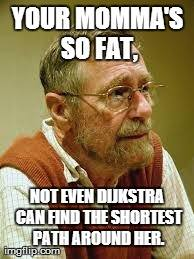
\includegraphics[width=7cm] {img/dijkstra.jpg}
    \end{center}
\end{figure}
\thispagestyle{empty}
\newpage
\pagenumbering{arabic}
\setcounter{page}{1}


\section{Introduction}
This is me trying to learn algdat. Credz to hakloev @ github for some of the content in this collection, pretty much or at least the stuff in norwegian and the pseudo code.


\section{Notation for asymptotic growth}


\begin{tabular}{|l|l|l|}
    \hline
    Name & Notation & Performance \\ \hline
    small-oh & $o(n)$ & $\textless n$ \\ \hline
    big-oh & $O(n)$ & $\le n$ \\ \hline
    theta & $\Theta(n)$ & $= n$ \\ \hline
    small omega & $\omega(n)$ & $\textgreater n$ \\ \hline
    big omega & $\Omega(n)$ & $\ge n$ \\ \hline
\end{tabular}


\section{Big-O Complexity Chart}
\begin{figure}[hbt]
    \begin{center}
        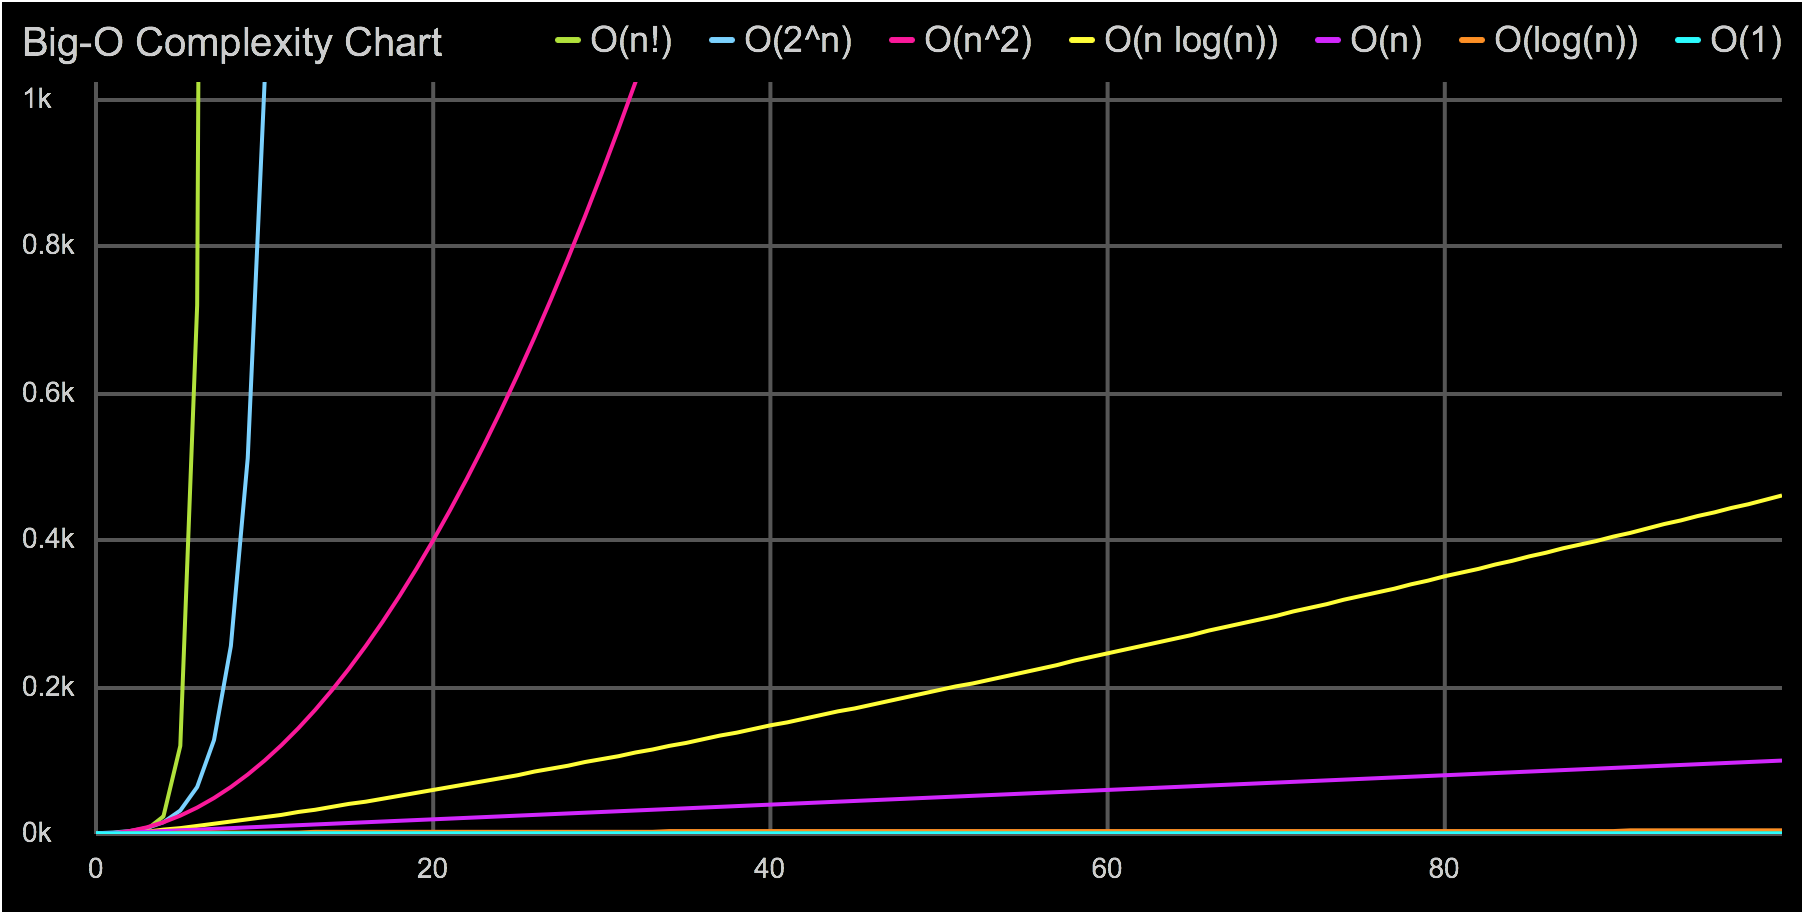
\includegraphics[width=12cm] {img/bigocomchart.png}
    \end{center}
\end{figure}

\newpage

\subsection{Complexity classes}


\begin{enumerate}
	\item Constant: $1$
	\item Polylogarithm: ${(log_{b}n})^{k}}$
	\item Polynominal: $n^k$
	\item Exponential: $2n$
	\item Factorial: $n!$
	\item Worse: $n^n$
\end{enumerate}

\subsection{Pseudopolynominal}

Gitt en algoritme som tar tallet $n$ som input og har kjøretid $O(n)$ – hvilken kompleksitetsklasse er dette? $n$ betegner her ikke størrelsen på input, men er selv en del av inputen. Det vil si at størrelsen til $n =$ antall bits som kreves $= lg(n)$. 

\begin{center}
$n = {2^{lg(n)}} = 2w \Rightarrow$ NB: Exponential time complexity! \
\end{center}

\section{Time Complexity}
\begin{tabular}{|l|l|l|l|}
	\hline
	Algorithm	            & Best & Average & Worst \\ \hline \hline \hline
	Insertion Sort          & $O(n)$ & $O(n^2)$ & $O(n^2)$ \\ \hline
	Heapsort                & $O(n log(n))$ & $O(n log(n))$ & $O(n log(n))$ \\ \hline
	Quicksort               & $O(n log(n))$ & $O(n log(n))$ & $O(n^2)$ \\ \hline
	Counting sort           & $O(n+k)$ & - & -  \\ \hline
	Radix sort              & $O(nk)$ & $O(nk)$ & $O(nk)$ \\ \hline
	Bucket sort             & $O(n+k)$ & $O(n+k)$ & $O(n^2)$ \\ \hline
	Topological sort (DFS)	& $O(V+E)$ & - & -  \\ \hline
	Bubble sort             & $O(n)$ & $O(n^2)$ & $O(n^2)$ \\ \hline
	Merge sort              & $O(n log(n))$ & $O(n log(n))$ & $O(n log(n))$ \\ \hline
	\hline
	BFS                     & $O(|E| + |V|)$ & - & - \\ \hline
	DFS                     & $O(|E| + |V|)$ & - & - \\ \hline
	Bellman-Ford            & $O(|V||E|)$ & - & - \\ \hline
	Dijkstra Heap           & $O((|V| + |E|) log |V|)$ & - & - \\ \hline
	Dijkstra Array          & $O(|V|^2)$ & - & - \\ \hline
	DAG-shortest (TP)       & $O(V+E)$ & - & -  \\ \hline
	Floyd-Warshall          & $O(V^3)$ - & - & - \\ \hline
	Binarysearch            & $O(log(n))$ & - & $O(log(n))$ \\ \hline
	\hline
	Ford-Fulkerson		    & $O(Ef)$ & $f = max flow of G$ & \\ \hline
	Edmons-Karp		        & $O(VE^2)$ & - & - \\ \hline
	\hline
	Huffman			        & $O(n log(n))$ & - & - \\ \hline
	\hline
	Kruskals			    & $O(E log(v))$ & - & - \\ \hline
	Prims			        & $O(E + V log(v))$ & - & - \\ \hline
	
\end{tabular}

\newpage


\section{Master method}

Masterteoremet er en form for ``kokebok''-metode for å løse rekurenser. Man kan som regel løse de fleste rekurrenser av typen: \\

\noindent $T(n) = aT(n/b) + f(n)$ hvor $a \ge 1$ og $b > 1$. $f(n)$ må også være asymptotisk positiv. \\ \hfill
\\ \hfill
Case 1: $f(n) = O(n^{log_{b}a - \varepsilon})$ , for en $\varepsilon > 0$ \\ \indent \indent \Rightarrow $T(n) = \Theta(n^{log_{b}a})$ \\
Case 2: $f(n) = \Theta(n^{log_{b}a})$  \\ \indent \indent \Rightarrow $T(n) = \Theta(n^{log_{b}a} log(n))$ \\
Case 3: $f(n) = \Omega(n^{log_{b}a + \varepsilon})$, for en $\varepsilon > 0$ og $af(n/b) \leq cf(n)$, hvor $c < 1$ \\ \indent \indent \Rightarrow $T(n) = \Theta(f(n))$

\newpage


\section{Datastructures}
\subsection{Array}
\subsubsection{Time complexity}
    \begin{tabular}{|l|l|l|l|}
    \hline
                        & Linked list       & Array    & Dynamic Array \\ \hline
    Indexing             & $\Theta(n)$          & $\Theta(1)$ & $\Theta(1)$      \\ \hline
    ins/del at beginning & $\Theta(1)$          & -        & $\Theta(n)$      \\ \hline
    ins/del at end       & $\Theta(n)$          & -        & $\Theta(1)$      \\ \hline
    ins/del at middle    & Search + $\Theta(1)$ & -        & $\Theta(n)$      \\ \hline
    wasted space         & $\Theta(n)$          & $0$        & $\Theta(n)$      \\ \hline
    \end{tabular}

\subsection{Heap}
A heap is a specialised tree-based data structure that satisfy the heap property.
There is no rules for how the siblings of a node is ordered in a heap.
A heap is often implemented as an Array. It is important that the key values from the heaps starts on the 2nd place in the array (index 1 in a 0-index array) to make it easier to calculate the siblings and parents of a node.

\subsubsection{Heap property}
If A is a parent node of B then the key of node A is ordered with respect to the key of node B with the same ordering applying across the heap. A heap has to have a full set of siblings for every node except the last one.\\

Min-heap:\\
The node with the smallest key value is always on the top of the heap. Every node beneath this node has a bigger key value and the nodes beneath the next node has even bigger. There can not be a node beneath another node with a smaller key value. \\


Max-heap:\\
This heap is the same as min-heap just reversed, with the biggest on top.

\begin{figure}[hbt]
    \begin{center}
        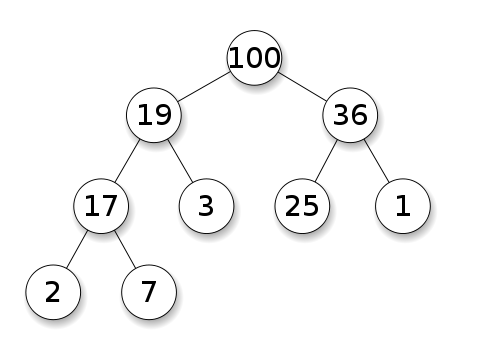
\includegraphics[width=5cm] {img/maxheap.png}
	\caption{A max-heep with integers between 1 and 100}
    \end{center}
\end{figure}

\subsubsection{Time complexity}
\begin{tabular}{|l|l|}
	\hline
	Operation      & Time complexity \\ \hline
	find-min/max   & $\Theta(1)$ \\ \hline
	delete-min/max & $\Theta(\log n)$ \\ \hline
	insert         & $\Theta(\log n)$               \\ \hline
	decrease-key   & $\Theta(\log n)$              \\ \hline
	merge          & $\Theta(n)$ \\ \hline
\end{tabular}\\
\textit{Note: that min/max depends on min/max heap}

\subsection{Stack}
Stack is a last in first out abstract data type. It is often implemented by using an array or a linked list. A stack uses operations as peek, push and pop.

\subsection{Queue}
Queue is a first in first out abstract data type. You can implement a queue by using an array (preferably a dynamic one) or a linked list. A queue uses operations as enqueue to put something in the queue, and dequeue to take it out.

\subsection{Binary Search tree}
Binary search tree is an ordered binary tree.

\subsubsection{Properties}
The left subtree of a node contains only nodes with keys less than the node's key.\\
The right subtree of a node contains only nodes with keys greater than the node's key.\\
The left and right subtree each must also be a binary search tree.\\
There must be no duplicate nodes.\\

\begin{figure}[hbt]
    \begin{center}
        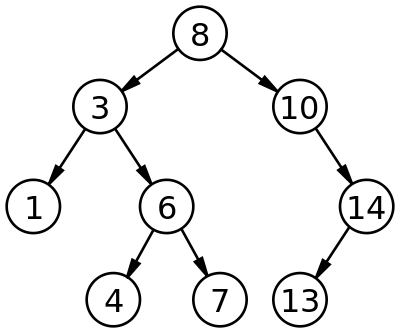
\includegraphics[width=5cm] {img/bst.png}
	\caption{A binary search tree of size 9 and depth 3}
    \end{center}
\end{figure}

\subsubsection{Time complexity}
\begin{tabular}{|l|l|l|}
    \hline
    Operation & Average & Worst \\ \hline
    Space     & $O(\log n)$       & $O(n)$     \\ \hline
    Search    & $O(\log n)$       & $O(n)$     \\ \hline
    Insert    & $O(\log n)$       & $O(n)$     \\ \hline
    Delete    & $O(\log n)$       & $O(n)$     \\ \hline
\end{tabular}
\subsection{Hash table}
Hash table or hash map is a data structure used to implement an associative array, a structure that can map keys to values. It works by taking a key and create an index by running it through a hashing algorithm. The index then can be used to find the correct value. The place where the value is stored is often called buckets or slots.
\subsubsection{Collisions}
The hash structure is very ideal for storing data very efficiently, but has some limitations. \\
The biggest problem is collisions, there is a possibility that the same hash is generated from two different keys, and therefor two keys can point at the same value. This is why it is important to have a good hashing algorithm.
\subsubsection{Perfect hashing}
Perfect hashing is not in the curriculum. The concept is built on that before building the hash table you know all the keys, and based on that knowledge you choose the perfect hashing algorithm. This will allowing you to get receive time complexity at linear time.
\subsubsection{Universal hashing}
Universal hashing is built on choosing a hashing algorithm at random for every key. This will in theory give you a very small collision rate, and in practice none.

\subsubsection{Time complexity}
\begin{tabular}{|l|l|l|}
    \hline
    Operation & Average & Worst \\ \hline
    Space     & $O(n)$       & $O(n)$     \\ \hline
    Search    & $O(1)$       & $O(n)$     \\ \hline
    Insert    & $O(1)$       & $O(n)$     \\ \hline
    Delete    & $O(1)$       & $O(n)$     \\ \hline
\end{tabular}
\subsection{Directed acyclic graph}

\begin{figure}[hbt]
    \begin{center}
        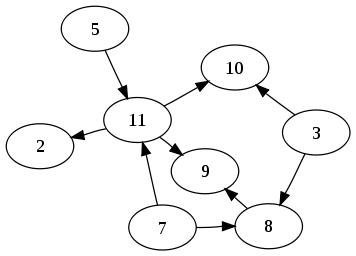
\includegraphics[width=5cm] {img/dag.png}
	\caption{An example of a directed acyclic graph}
    \end{center}
\end{figure}


\subsection{Adjacency matrix}
\subsection{Representation of graphs}




\section{Searching algorithms}
\subsection{Breadth-first search}
BFS is a strategic algorithm for searching a graph. It has only two operations which is \textit{visit and inspect a node} and \textit{gain access to visit the nodes that is the neighbor of the currently visited node}
It can be used to find shortest path. 
BFS uses a queue to keep track of what nodes to visit.
\\
\begin{algorithmic}
\Function{BFS}{$G, v$} \Comment v er startnode 
        \State lag en kø $Q$
        \State legg $v$ inn i $Q$
        \While {$Q.notEmpty()$}
                \State $v = Q.dequeue()$
                \For {each edge $e$ adjacent to $v$}
                        \If {$e$ not marked}
                                \State mark $w$
                                \State $Q.enqueue(e)$
                        \EndIf
                \EndFor
        \EndWhile
\EndFunction

\begin{figure}[hbt]
    \begin{center}
        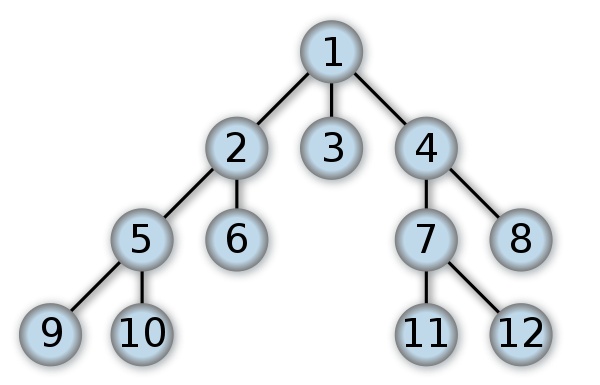
\includegraphics[width=5cm] {img/bfs.png}
	\caption{A graph with example of the bfs visit order}
    \end{center}
\end{figure}

\subsection{Depth-first search}
DFS is like BFS an algorithm to search a graph. Instead of a queue, DFS uses a stack and it can be implemented recursively.
A directed graph can contain forward edge, backward edge, cross edge and tree edge.
A undirected graph can contain backward and cross edge
\\

\begin{algorithmic}
\Function{DFS}{$G, v$} \Comment v er startnode
        \State initaliser en tom stack, $S$
        \For {each vertex $u$ in G}
        \State set $visited[u] \rightarrow false$
        \EndFor 
        \State $S.push(v)$
        \While{$S.notEmpty()$}
                \State $u = S.pop()$
                \For {all $w$ adjacent to $u$}
                        \If {not $visited[w]$}
                                \State $visited[w] \rightarrow true$
                                \State $S.push(w)$
                        \EndIf
                \EndFor
        \EndWhile
\EndFunction
\end{algorithmic}

\\ maybe talk about all the edgetypes?
\begin{figure}[hbt]
    \begin{center}
        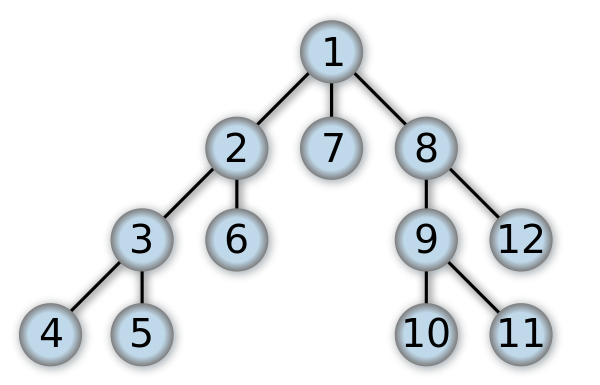
\includegraphics[width=5cm] {img/dfs.png}
	\caption{A graph with example of the dfs visit order}
    \end{center}
\end{figure}

\subsection{Bellman-Ford algorithm}
Bellman-Ford is an single-source shortest path algorithm. It is slower than Dijkstra, because it can detect negative cycles by running an additional check. If it detect a negative cycle it returns a false or an error. It is built upon the principle of relaxation, in which an approximation to the correct distance is gradually replaced by a more accurate values until eventually reaching the optimal solution. Bellman-ford is not a greedy algorithm like Dijkstra, instead it checks every outgoing edge form a node.4
\\

\begin{algoritmic}
\Function{BELLMANN-FORD}{$G, w, s$}
\State \Call{INITIALIZE-SINGLE-SOURCE}{$G, s$}
\For {$i = 1$ to $|G.V| - 1$}
        \For {each edge $(u, v) \in G.E$}
                \State \Call{RELAX}{$u, v, w$}
        \EndFor
\EndFor
\For {each edge $(u, v) \in G.E$}
        \If {$v.d > u.d + w(u, v)$}
                \State \Return $false$
        \EndIf
\EndFor
\State \Return $true$
\EndFunction

\end{algoritmic}

\subsection{DAG-shortest path}
The idea of DAG-shortest path is to use Topological sort on the graph to find the topological sorting of the graph represented in linear ordering. Once we have a linear presentation we can processes every vertex one by one and update the distance using the value of the current vertex.
\\

\begin{algoritmic}
\Function{DAG-SHORTEST-PATH}{G, w, s}
\State \Call{TOPOLOGICAL-SORT}{G}
\State \Call{INITIALIZE-SINGLE-SOURCE}{G, s}
\For {each vertex $u$, taken in topologically sorted order}
        \For {each vertex $v \in G.Adj[u]$}
                \State \Call{RELAX}{u, v, w}
        \EndFor
\EndFor
\EndFunction
\end{algoritmic}

\subsection{Dijkstra's algorithm}
Dijkstra's shortest path algorithm is faster than Bellman-Ford because it do expect that the graph has no negative cycle. Because of this, it will not work on graphs with negative cycle and it will not finish. \\
Dijkstra can be implemented with an ordinary array as priority queue., but will den not achieve that great time complexity. If it is implemented with a min-heap or a Fibonacci-heap then you can receive great time complexity.
\\

\begin{algoritmic}
\Function{DIJKSTRA}{$G, w, s$}
\State \Call{INITIALIZE-SINGLE-SOURCE}{$G, s$}
\State $S = \emptyset$
\State $Q = G.V$
\While {$Q \neq \emptyset$}
        \State $u = $ \Call{EXTRACT-MIN}{Q}
        \State $S = S \cup \{u\}$
        \For {each vertex $v \in G.Adj[u]$}
                \State \Call{RELAX}{u, v, w}
        \EndFor
\EndWhile
\EndFunction

\end{algoritmic}

\subsection{Floyd-Warshall algorithm}
Floyd-Warshall is an algorithm for finding all to all shortest path. It is an example of dynamic programming. By default it only finds the shortest way by value, not by weight. It is possible to write the algorithm with path reconstruction.
\\

\begin{algoritmic}
\Function{FLOYD-WARSHALL}{$W$}
\State ${D^{(0)} = W$
\For {$k = 1$ to $n$}
        \State let ${D^{(k)}$ be a $n$ x $n$ matrix
        \For {$i = 1$ to $n$}
                \For {$j = 1$ to $n$}
                        \State ${D_{ij}^{(k)} = min(${D_{ij}^{(k-1)}, {D_{ik}^{(k-1)} + {D_{kj}^{(k-1)})$
                \EndFor
        \EndFor
\EndFor
\State \Return ${D^{(n)}$
\EndFunction

\end{algoritmic}

\subsection{Binary search}
In computer science, a binary search or half-interval search algorithm finds the position of a specified input value (the search "key") within an array sorted by key value. In each step, the algorithm compares the search key value with the key value of the middle element of the array. If the keys match, then a matching element has been found and its index, or position, is returned.

\section{Flow networks}
\subsection{Ford-Fulkerson method}
Ford-Fulkerson is an algorithm/method which computes the maximum flow in a flow network. \\
The idea behind the algorithm is as follows: As long as there is a path from the source (start node) to the sink (end node), with available capacity on all edges in the path, we send flow along one of these paths. Then we find another path, and so on. A path with available capacity is called an augmenting path.
The algorithm uses DFS to find the augmenting path
\subsubsection{Augmented path}
An augmenting path is simply a path through the graph using only edges with positive capacity from the source to the sink.
\subsection{Edmonds-Karp}
It is exactly the same as Ford-Fulkerson, but instead of using DFS  it uses BFS.


\section{Sorting algorithms}
\subsection{Insertion Sort}
Insertion sort is a simple sorting algorithm which sorts items one at a time. It is not efficient, but has advantages as simple implementation, efficient for small data sets and stable.
\\

\begin{algorithmic}
\For {$j=0$ to $A.length$}
        \State $key = A[j]$ 
        \State $i = j - 1$ 
        \While {$i > 0$ and $A[i] > key$}
                \State $A[i + 1] = A[i]$ 
                \State $i = i - 1$ 
        \EndWhile
        \State $A[i] + 1 = key$ 
\EndFor
\end{algorithmic}


\subsection{Heapsort}
Heapsort is a comparison-based sorting algorithm to create a sorted array. The algorithm works in two parts. The first part is to build a heap out of the data. \\
The second part is taking out the biggest element of the heap and putting it into an array as long as there is still items in the heap. The heap is reconstructed every time. The order of the sorted array as a result is based on if the heap was a max heap or a min heap.
\\

\begin{algorithmic}
\State \Call{BUILDMAXHEAP}{$A$} 
\For {$i = A.length$ downto $2$}
        \State exchange $A[1]$ with $A[i]$
        \State $A.heapSize$ = $A.heapSize -1$
        \State \Call{MAX-HEAPIFY}{$A, 1$} 
\EndFor
\end{algorithmic}

\subsection{Quicksort}
Quicksort is one of the most used sorting algorithm and is on the average case very fast. It is a divide and conquer sorting algorithm which working in the following way: \\\\ 
Step 1: Pick an element, called a pivot element from the list to be sorted.\\
Step 2: Reorder the list so that all elements with value less than the pivot come before the pivot and all bigger come after. After this, the pivot is on its final position. This is called the partition operation.\\
Step 3: Recursively apply the above steps to the sublist now created on the sides of the pivot element.
\\\\
Quicksort is often depended on choosing a good pivot element to have good time complexity. This is often solved by choosing one at random.
\\

\begin{algorithmic}
\Function{QUICKSORT}{$A, p, r$}
\If {$p < r$}
        \State $q$ = \Call{PARTITION}{$A, p , r$}
        \State \Call{QUICKSORT}{$A, p, q -1$}
        \State \Call{QUICKSORT}{$A. q + 1, r$}
\EndIf
\EndFunction \\

\Function{PARTITION}{$A, p, r$}
        \State $x = A[r]$
        \State $i = p - 1$
        \For {$j = p$ to $r -1$}
                \If {$A[j] \leq x$}
                        \State $i = i + 1$
                        \State exchange $A[i]$ with $A[j]$
                \EndIf
        \EndFor
\State exchange $A[i + 1]$ with $A[j]$
\State \Return{$i + 1$}
\EndFunction
\end{algorithmic}

\subsection{Counting sort}
Counting sort is a sorting algorithm that can sort only whole integers and is therefor a integer sorting algorithm. It counts the amount of time a integer or key is in an array and then fill in the amount of times the integer appears in the index of the integers value in the counting array. After the counting array is done, it will adjust the counting array so that the value of an index represent the index of the final index in the final sorted array.
Counting sort is often used as a subroutine in algorithms such as Radix sort.
\\

\begin{algorithmic}
\Function{COUNTINGSORT}{$A, B, k$}
\State let $C[0 \dots k]$ be a new array
\For {$i=0$ to $k$}
\State $C[i]=0$
\EndFor
\For {$j=1$ to $A.length$}
\State $C[A[j]] = C[A[j]] + 1$
\EndFor
\For {$i=0$ to $k$}
\State $C[i] = C[i] + C[i -1]$
\EndFor
\For {$j=A.length$ downto $1$}
\State $B[C[A[j]]] = A[j]$
\State $C[A[j]] = C[A[j]] - 1$
\EndFor
\EndFunction
\end{algorithmic}

\subsection{Radix sort}
Radix sort is a sorting algorithm that sorts data based on a part-value at a position in the value. It sorts first by the part-value at place -1 and from there it goes to -2 and so on. It uses counting sort for the sorting operation.
\\

\begin{algorithmic}
\Function{RADIXSORT}{$A, d$}
\For {$i = 1$ to $d$}
        \State Bruk \textit{Stable Sort} til å sortere array $A$
\EndFor
\EndFunction 
\end{algorithmic}

\subsection{Bucket sort}
Bucket sort that works by partitioning an array into a number of buckets. After the initial sorting, the buckets are sorted individually, by applying bucket sort again or by using another sorting algorithm.
\\

\begin{algorithmic}
\Function{BUCKETSORT}{$A$}
\State $n = A.length$
\State la $B[0 \dots n - 1]$ være et nytt array
\For {$i = 0 $ to $n - 1$}
        \State Gjør $B[i]$ til en tom liste
\EndFor
\For {$i = 1$ to $n$}
        \State Sett inn $A[i]$ i lista $B[ \lfloor nA[i] \rfloor ]$
\EndFor
\For {$i = 0$ to $n - 1$}
        \State Sorter lista $B[i]$ med \Call{InsertionSort}{B[i]} 
\EndFor
\State Konkatiner listene $B[0], B[1], \dots , B[n - 1]$ i rekkefølge
\EndFunction 
\end{algorithmic}

\begin{figure}[hbt]
    \begin{center}
        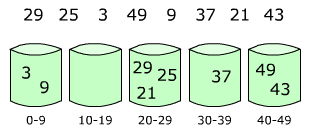
\includegraphics[width=5cm] {img/unsortedbucket.png}
	\caption{Some unsorted buckets}
    \end{center}
\end{figure}
\begin{figure}[hbt]
    \begin{center}
        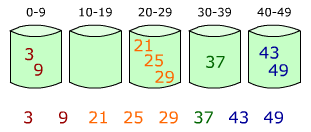
\includegraphics[width=5cm] {img/sortedbucket.png}
	\caption{Some sorted buckets}
    \end{center}
\end{figure}
\subsection{Topological sort}
Topological sort is a linear ordering of a directed acyclic graphs vertices. One way to topological sort is to use an algorithm based on DFS. Every DAG has at least one topological sort.
\\

\begin{algorithmic}
\Function{TOPOLOGICALSORT}{$G$}
\State \Call{DFS}{$G$} to compute finish times $v.f$ for each vertex $v$.
\State as each vertex is finished, insert it onto the end of the list
\State \Return{the list of verticies}
\EndFunction
\end{algorithmic}

\subsection{Bubble sort}
Bubble sort is a simple sorting algorithm that works by repeatedly stepping through the list to be sorted, comparing each pair of adjacent items and swapping them if they are in the wrong order. The pass through the list is repeated until no swaps are needed, which indicates that the list is sorted. 
\begin{algorithmic}
\For {$i=0$ to $A.length - 1$}
        \For {$j=A.length$ downto $i + 1$}
                \If {$A[j] < A[j -1]$}
                        \State exchange $A[j]$ with $A[j-1]$
                \EndIf
        \EndFor
\EndFor
\end{algorithmic}
\subsection{Merge sort}
Merge sort is a divide and conquer sorting algorithm that splits a list in two and then calls itself recursively. When every list is a single element list, it will start the merge part where it merges the list back together in sorted order.
\\

\begin{algorithmic}
 \Function{MERGE-SORT}{$A, p, r$} 
        \If {$p < r$}
                \State $q = \lfloor(p + r) / 2 \rfloor $ 
                \State \Call{MERGE-SORT}{$A, p, q$} 
                \State \Call{MERGE-SORT}{$A, q + 1, r$}
                \State \Call{MERGE}{$A, p, q, r$} 
         \EndIf
\EndFunction
\State 

\Function{MERGE}{A, p, q, r}
\State ${n_{1}}=q-pr+1$
\State ${n_{2}}=r-q$
\State let $L[1 \dots {n_{1}} + 1]$ and $R[1 \dots {n_{2}+1}$ be new arrays
\For {$i=1$ to ${n_{1}}$}
        \State $L[i] = A[p + i -1]$
\EndFor
\For {$j=1$ to ${n_{2}}$}
        \State $R[j] = A[q + j]$
\EndFor
\State $L[{n_{1}}] + 1] = \infty$
\State $r[{n_{2}}] + 1] = \infty$
\State $i = 1$
\State $j = 1$
\For {$k=p$ to $r$}
        \If {$L[i] \leq R[j]$}
                \State $A[k] = L[i]$
                \State $i = i + 1$
        \Else 
                \If  {$A[k] = R[j]$}
                        \State $j = j + 1$
                \EndIf        
        \EndIf
\EndFor
\EndFunction
\end{algorithmic}


\subsection{Huffman}

\section{Dynamic Programming}
Overlapping part problem and Optimal substructure. If a locally optimal problem is a global solution, then it is a optimally global problem, then you can use greedy algorithm.\\
DP = memoising, recursion and guessing.\\
Dynamic programming is pretty much shortest path with DAG.\\

\subsection{Five easy steps to DP}
\begin{enumerate}
	\item Define subproblems
	\item Guess (part of solution)
	\item Relate subproblem solutions
	\item Recurse and memoize\\ or\\ Build DP table bottom-up
	\item Solve original problem
\end{enumerate}

\subsection{Memoising}
For memoising to work, the problem need to be acyclic, else it will run infinite.
\subsection{Rod cutting}
\subsection{Matrix-chain multiplication}

\section{Greedy algorithm}
\subsection{Huffman}

\section{Minimal spanning trees}
\subsection{Growing a minimal spanning tree}
\subsection{Kruskals algorithm}

Kruskals algoritme sorterer alle kanter etter kostnaden og velger den billigste tilgjengelige kanten , og legger til denne med noder i treet. Dette kun hvis den ikke allerede er brukt og vil danne en sykel. Fortsetter til det ikke finnes kanter som kan legges til i treet.  \\ \hfill
\\

\begin{algoritmic}
\Function {KRUSKAL}{G, w}
\State $A = \emptyset$
\For {each vertex $v \in G.V$}
        \State \Call{MAKE-SET}{$v$}
\EndFor
\State sort edges of $G.E$ into nondecreasing order by weight $w$
\For {each edge $(u,v) \in G.E$, taken in nondecreasing order by weight}
        \If {\Call{FIND-SET}{$u$} $\neq$ \Call{FIND-SET}{$v$}}
                \State $A = A \cup \{ (u,v) \}$
                \State \Call{UNION}{u,v} 
        \EndIf  
\EndFor
\State \Return{$A$}


\subsection{Prims algorithm}

Prims algoritme velger en tilfeldig node, og legger alle kantene inn i en prioritetskø etter vekt. Velger den billigste kanten og legger den til i treet.  Det vil si at den legger til den billigste kanten som er mulig å legge til fra treet den bygger. \\ \hfill
\\

\begin{algoritmic}
\Function {PRIM}{G, w, r}
\For {each $u \in G.V$}
        \State $u.key = \infty$
        \State $u.\pi = NIL$
\EndFor
\State $r.key = 0$
\State $Q = G.V$
\While {$Q \neq \emptyset$}
        \State $u = \Call{EXTRACT-MIN}{Q}$
        \For {each $v \in G.Adj[u]$}
                \If {$v \in Q$ and $w(u, v) < v.key$}
                        \State $v.\pi = u$
                        \State $v.key = w(u, v)$
                \EndIf
        \EndFor
\EndWhile
\EndFunction
\end{algoritmic}


\section{NP}
\subsection{Reduction}
If you have A and B, and A is a known hard problem, and you want to show that B is a hard problem, then you can reduce A to B to show that B is a hard problem.
If a problem is in both NP and NP-Hard then it is NPC (NP Complete)

\section{NP-Komplette problemer}

\noindent NP $\Rightarrow$ Nondeterministic Polynomial \\
\noindent NPC $\Rightarrow$ NP-Complete\\
\noindent P $\Rightarrow$ Polynomial \\ \\

\noindent \textbf{Sammenhengen mellom alle NP-problemer:} \\

$P \subseteq NP$ \\
$NPC \subseteq NP$ \\ \\

\noindent Hvis et problem $A \in NPC$, så vil også $A \in NP$. Dette er fordi $NP = P + NPC$. Hvis noe ikke er i P eller NPC, er det heller ikke i NP, fordi $P \cap NPC = \emptyset$. \\ \hfill
\begin{figure}[hbt]
    \begin{center}
        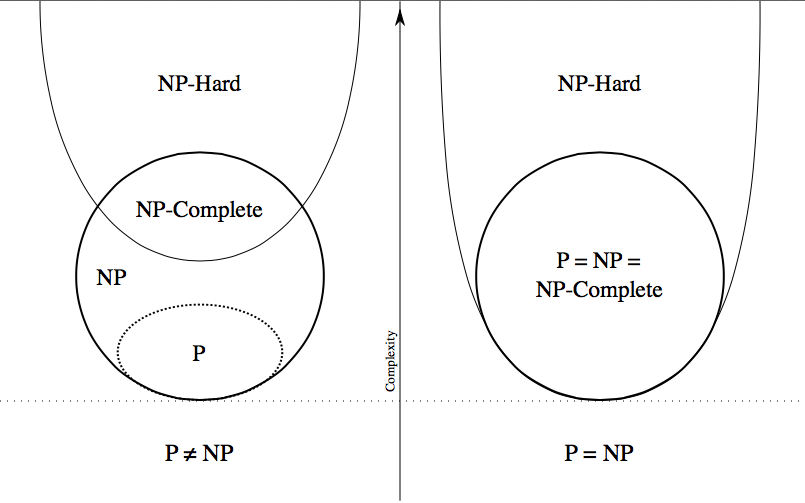
\includegraphics[width=7cm] {npc.png}
        \caption{Venndiagramet, med med $P \neq NP$ og $P = NP$}
    \end{center}
\end{figure}

\noindent Du vet at problem A er i NP og problem B er i NPC. Du vil vise at A også er i NPC. Da reduserer du fra B til A.\\ \hfill

\noindent Du står overfor de tre problemene A, B og C. Alle tre befinner seg i mengden NP. Du vet at A er i mengden P og at B er i mengden NPC. Anta at du skal bruke polynomiske reduksjoner mellom disse problemene til å vise $\dots$:

\begin{enumerate}
        \item $\dots$ at C er i P må $C \leq A$ (C reduseres til A)
        \item $\dots$ at C er i NPC må $B \leq C$ (B reduseres til C)
        \item $\dots$ hvis B kan reduseres til A er $P = NP$ (NB: ikke løst enda)
        \item Alle disse reduksjonene skjer i polynomisk tid
\end{enumerate}

\noindent To ikke helt legitime, men greie huskeregeler: 
\begin{center}
\textit{reduser fra litt til mer // fra litt \dots $\leq$ \dots til mer\\ }
\textit{reduser nedover: NPC $\rightarrow$ (NP) $\rightarrow$ P (forsiktig med denne)\\ \hfill}
\end{center}

\begin{figure}[hbt]
    \begin{center}
        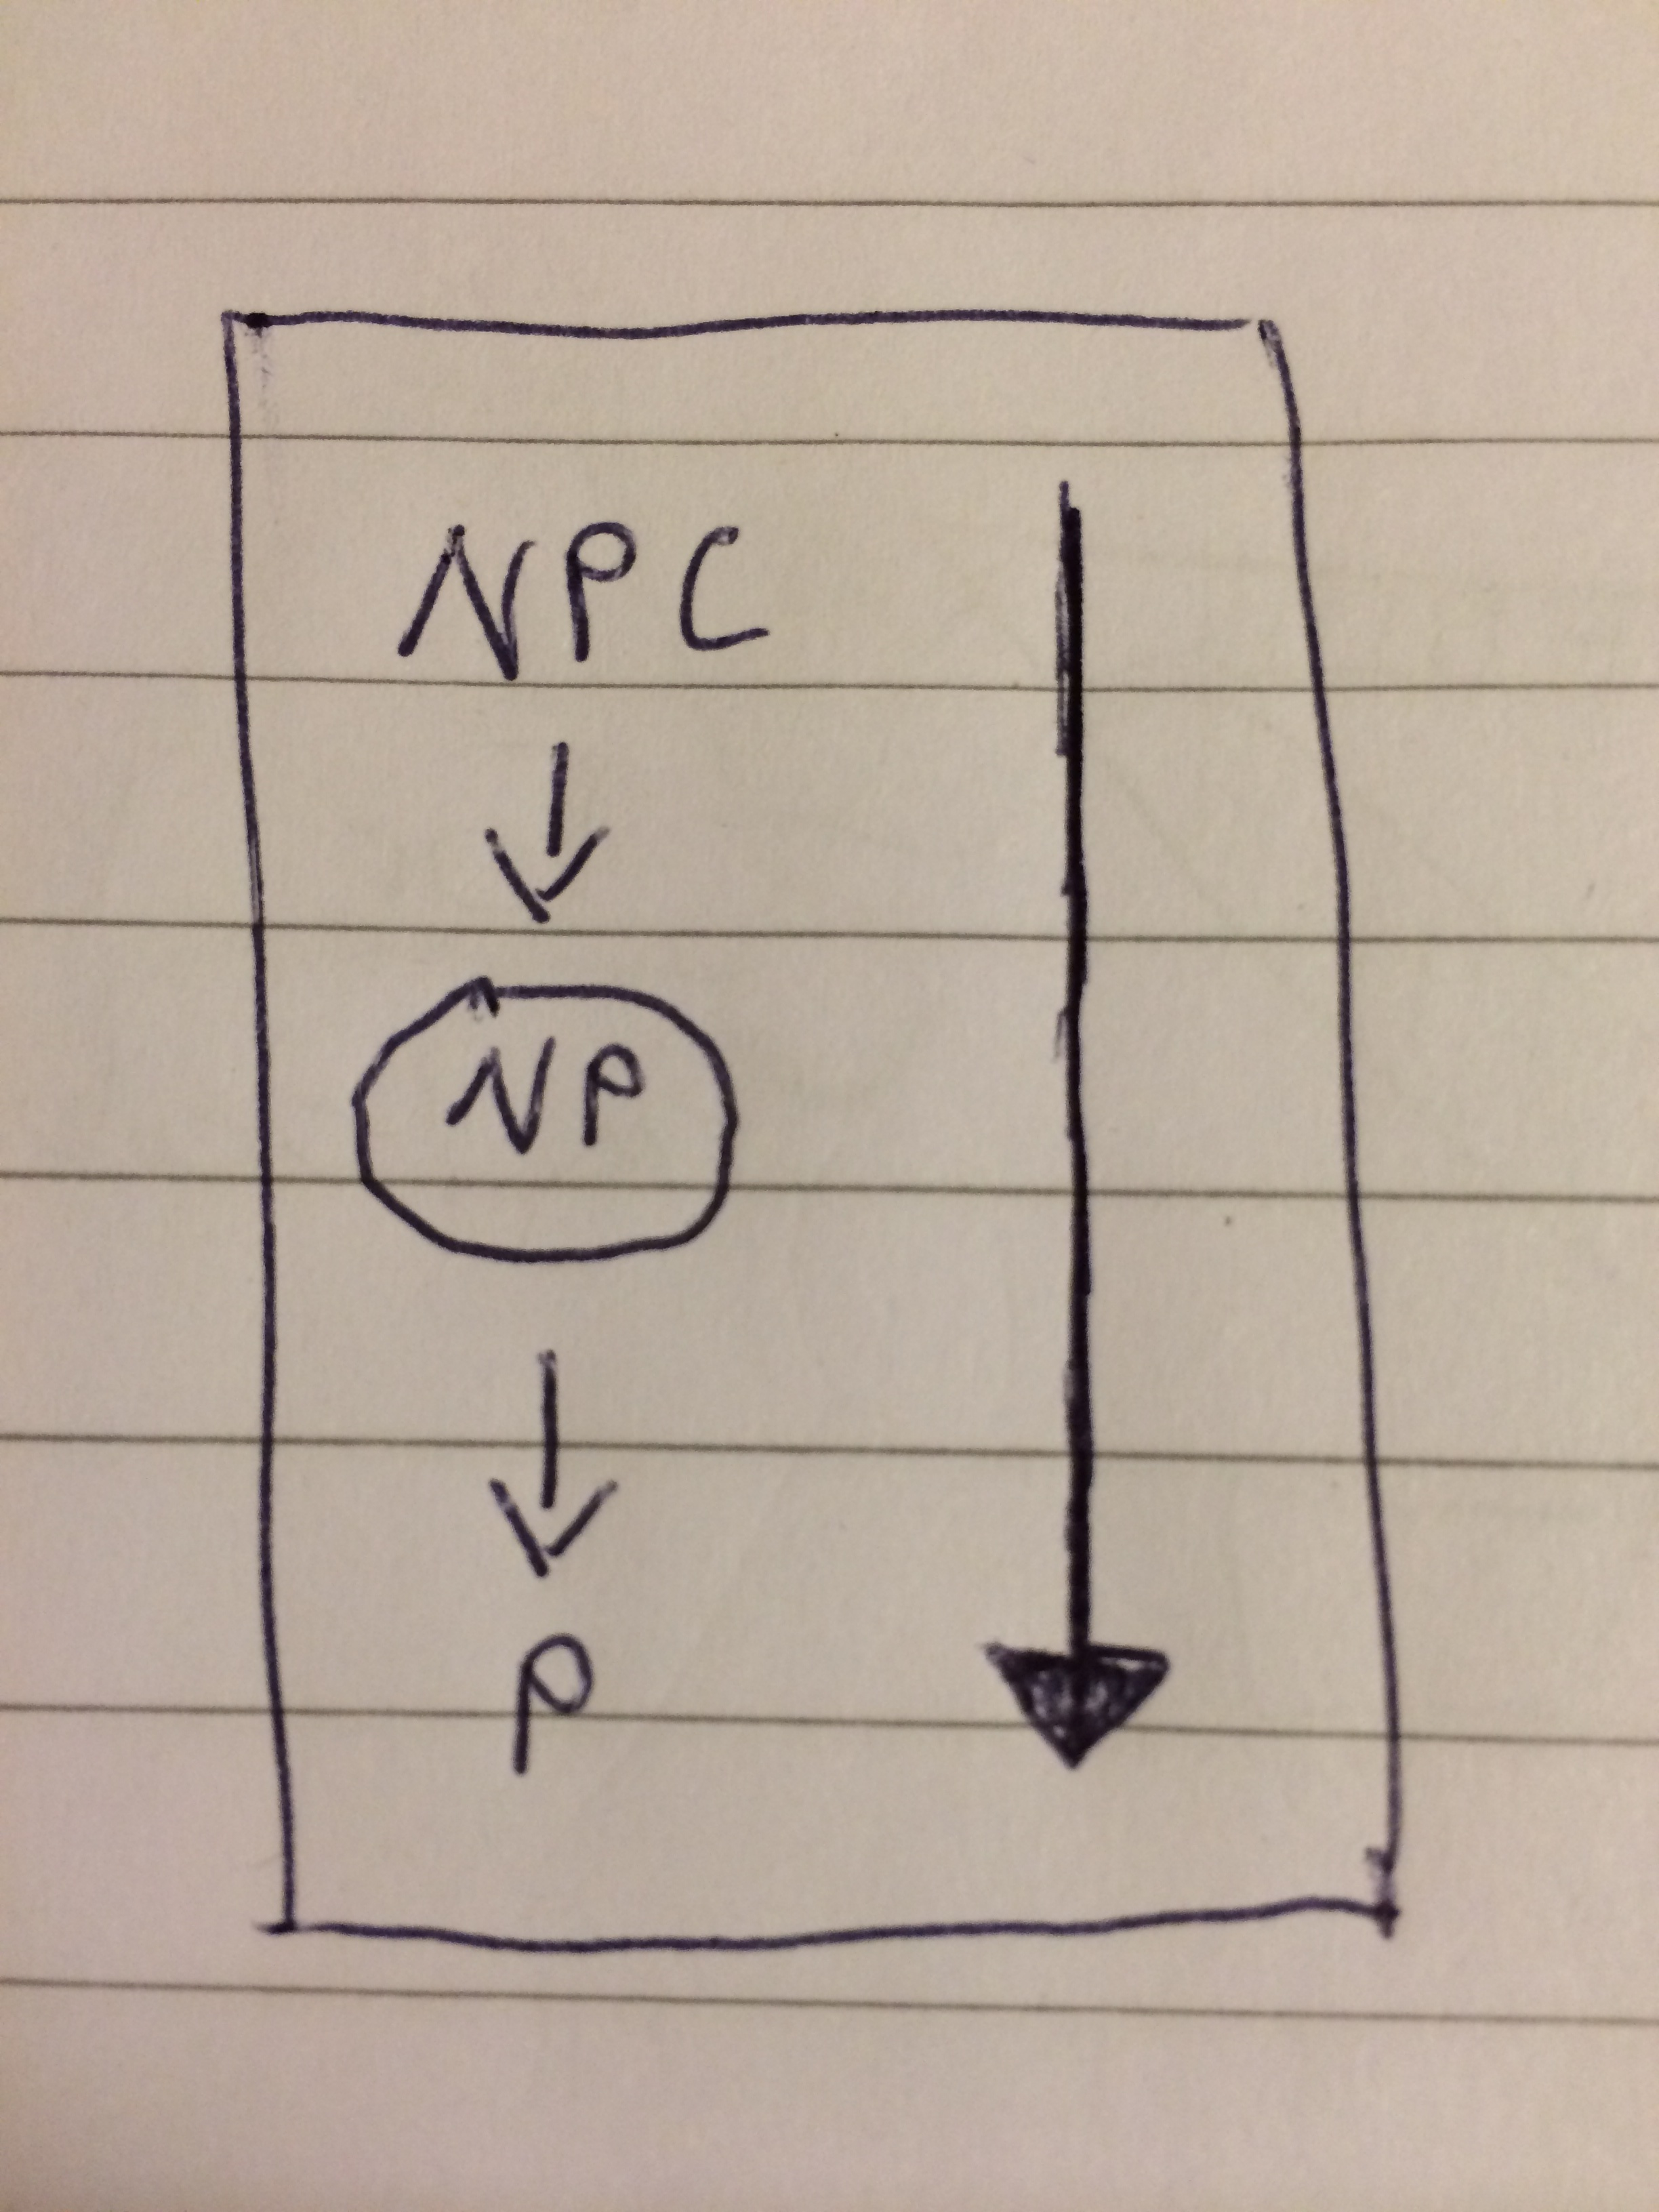
\includegraphics[width=3cm] {cheat.jpg}
        \caption{En tvilsom huskeregel, NB!}
    \end{center}
\end{figure}

\noindent \textbf{Liste/strukturen til NPC-problemer redusert fra CIRCUT-SAT:}

\begin{itemize}
\item CIRCUT-SAT
\item SAT
\item 3-CNF-SAT
        \begin{itemize}
                \item SUBSET-SUM
                \item CLIQUE
                \begin{itemize}
                                \item VERTEX-COVER
                                \item HAM-CYCLE
                                \item TSP (Traveling Salesman Problem)
                \end{itemize}
        \end{itemize}
\end{itemize}


\end{document}


